\documentclass[a4paper]{article}
\usepackage{graphicx}
\usepackage{wrapfig}
\usepackage{caption}
\usepackage{subcaption}
\usepackage{amsfonts} 


\title{Quick Sort}
\author{Yarne Ramakers}
\date{\today}

\begin{document}

%\maketitle - had to comment as it took up too much space
\begin{center}
  Quicksort \\
  Yarne Ramakers \\
  \today \\
\end{center}

\begin{figure}[h]
  \begin{subfigure}{0.3\textwidth}
    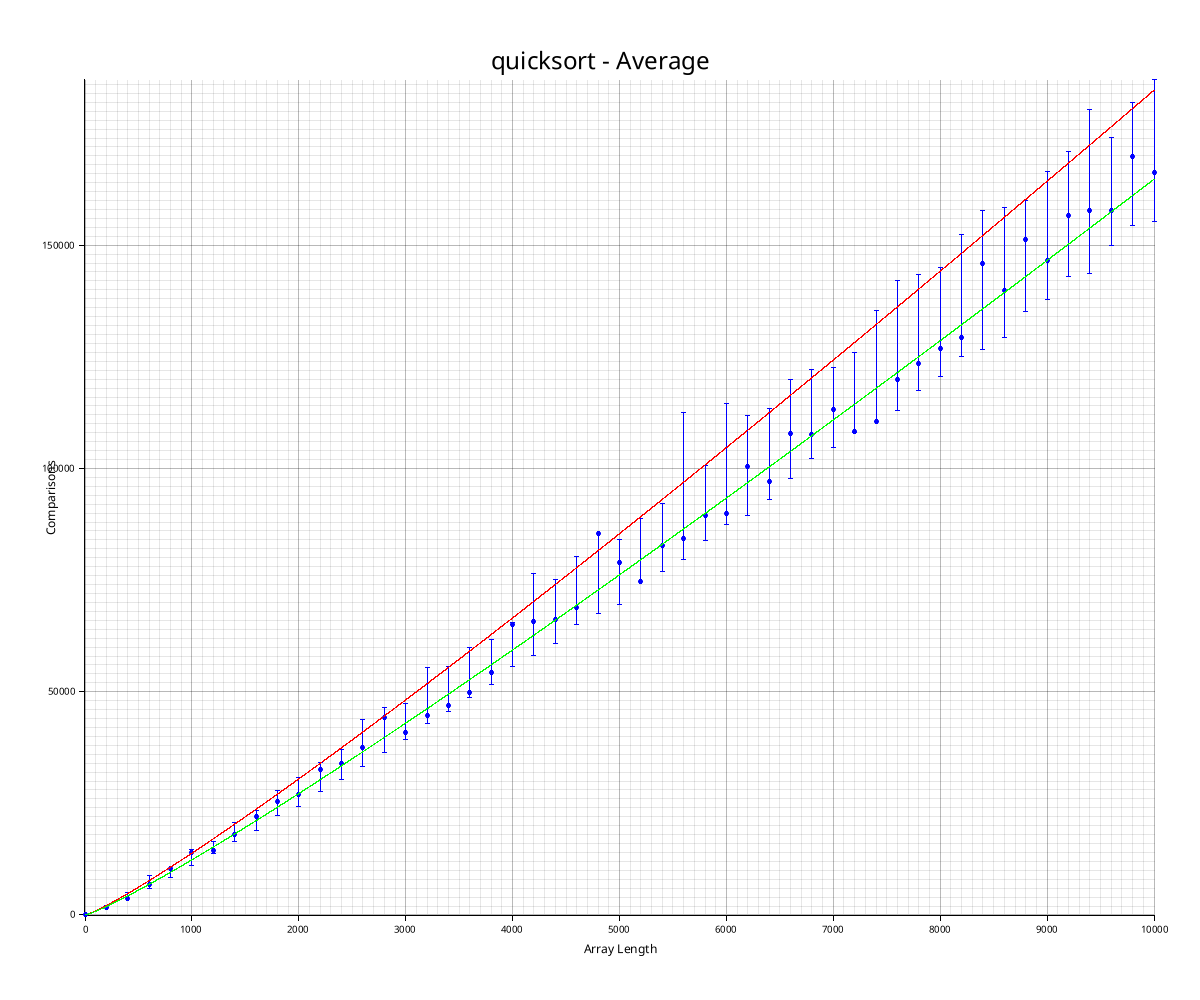
\includegraphics[width=\textwidth]{../plots/quicksort-average.png}
    \caption{Average case}
    \label{fig:merge-avg}
  \end{subfigure}
  \begin{subfigure}[b]{0.3\textwidth}
    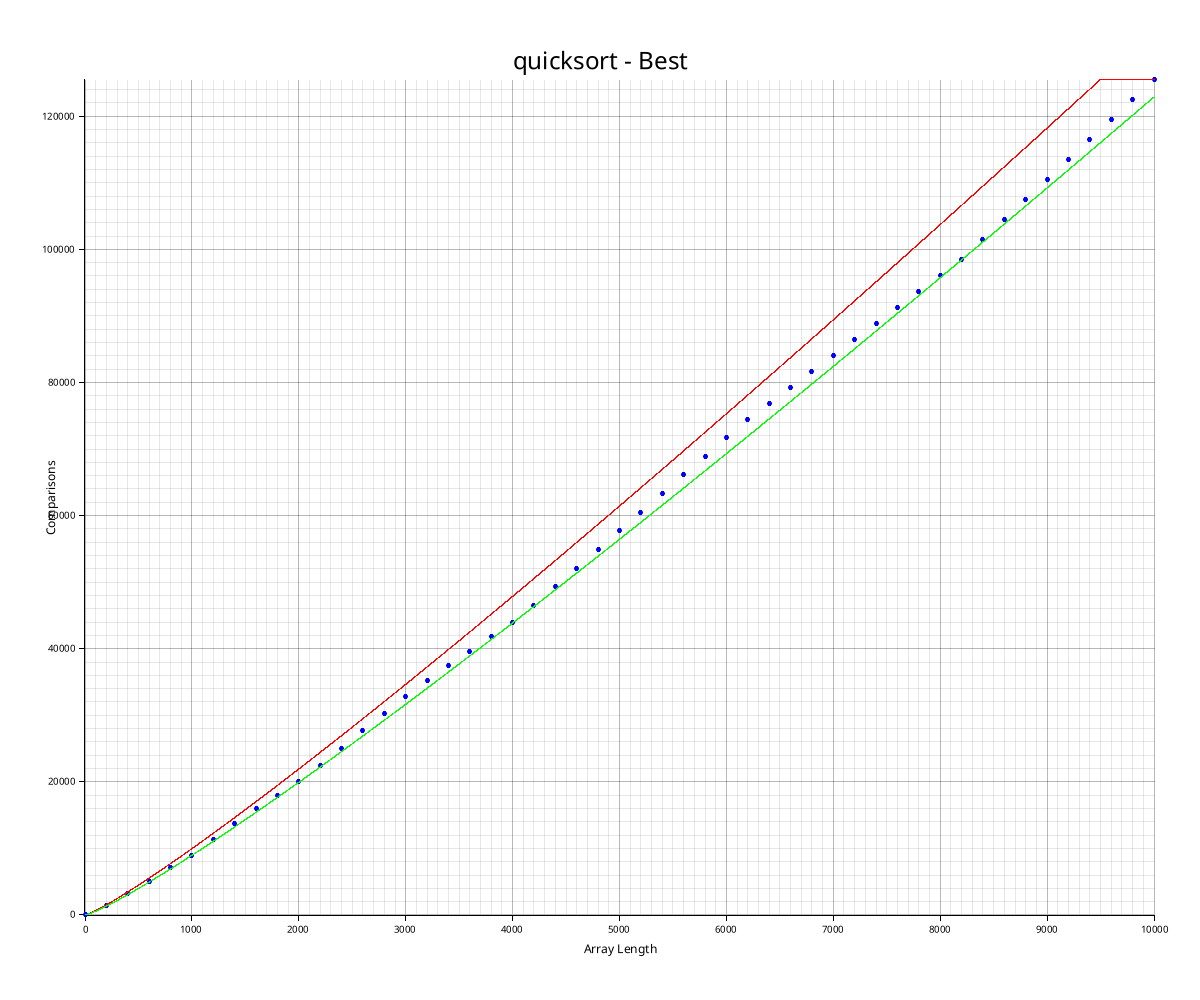
\includegraphics[width=\textwidth]{../plots/quicksort-best.png}
    \caption{Best case}
    \label{fig:merge-best}
  \end{subfigure}
  \begin{subfigure}[b]{0.3\textwidth}
    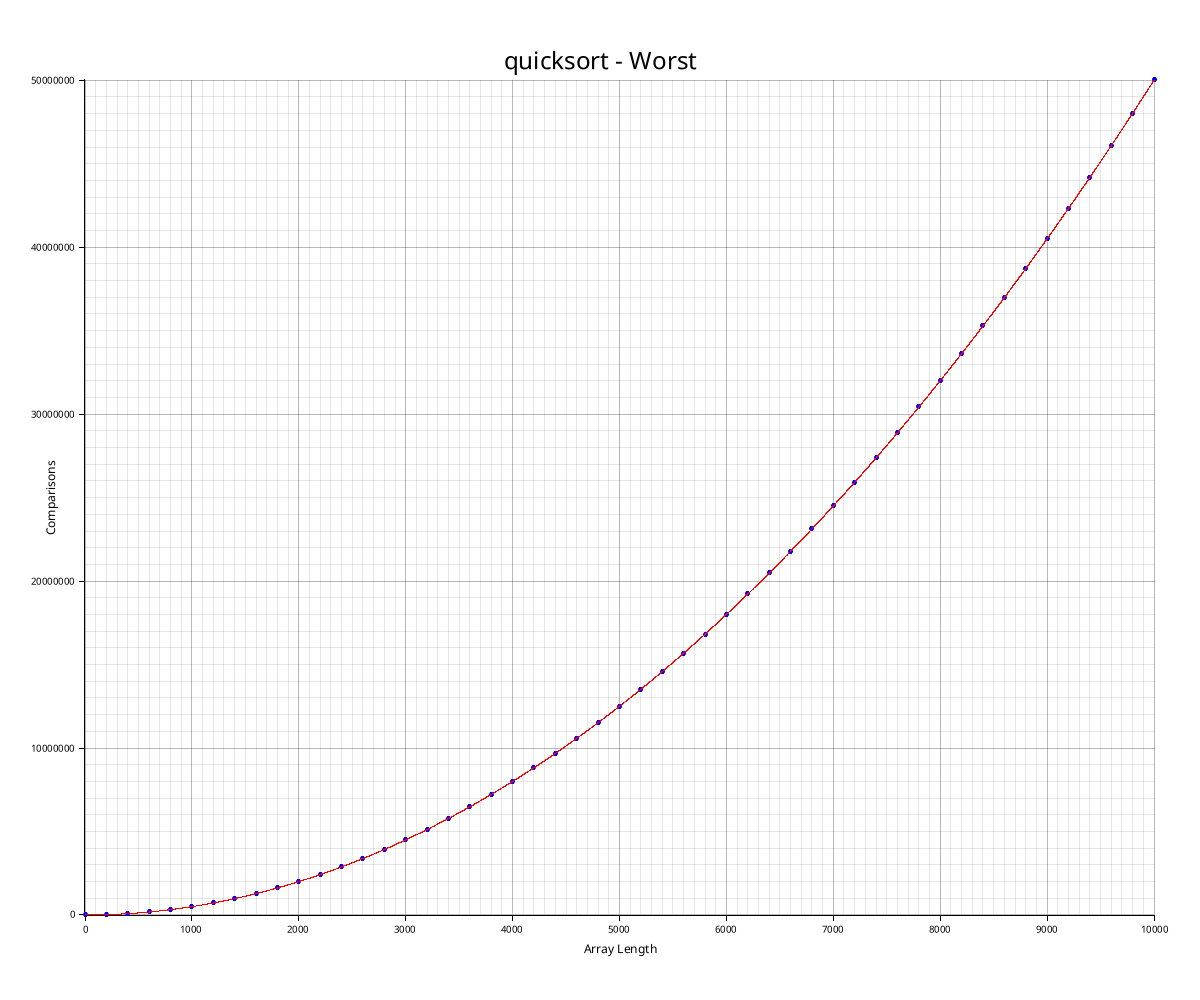
\includegraphics[width=\textwidth]{../plots/quicksort-worst.png}
    \caption{Worst case}
    \label{fig:merge-worst}
  \end{subfigure}
\end{figure}

\section{Introductie}
% Introduction to merge sort and its importance.
Quicksort is een sorteeralgoritme dat gebruik maakt van het verdeel en heers principe.
Het is een van de snelste sorteeralgoritmes en wordt vaak gebruikt in de praktijk.

\section{Bevindingen}
% Discuss the results of the experiments.
Ik heb quicksort in rust ge\"implementeerd met Hoare's partitie en getest op verschillende soorten lijsten.
De grafieken \ref{fig:merge-best} en \ref{fig:merge-worst} tonen de theoretische complexiteit van quicksort in best case en worst case respectievelijk.
De rode lijn toont de theoretische complexiteit van quicksort, namelijk $\sim n \log n$ en $\sim n^2$ respectievelijk.
De blauwe punten tonen de gemeten vergelijkingen over lijsten voor verschillende lengte $n$. 
We merken op dat bij de best case de metingen onder the theoretische complexiteit liggen. Dit komt omdat $\sim n \log n$ een bovengrens is.
De werkelijke complexiteit is $n \log n - n + 1$ deze complexiteit wordt voorgesteld door de groene lijn.
\par
De grafiek \ref{fig:merge-avg} toont de theoretische complexiteit van quicksort in het gemiddelde geval.
We weten dat dit gedrag tussen $\sim n \log n$ en $\sim n^2$ zal liggen. Dit zal dus gelijk zijn aan $\sim cn \log n$. Met $1<c<2^n$.
Omdat dit voor elke lijst moet gelden zal $1<c<2$ zijn. In de les hebben we deze $c$ bepaald als $1.39$. Op de grafiek \ref{fig:merge-avg} stelt de rode lijn de theoretische complexiteit voor, namelijk $\sim 1.39n \log n$.
We merken echter dat de gemeten complexiteit onder deze theoretische complexiteit ligt. Dit komt omdat we bij het bereken van de complexiteit de overhead van het meten niet hebben meegenomen.
Volgens mijn programma ligt de werkelijke complexiteit op ongeveer $1.24n \log n$ dit wordt voorgesteld door de groene lijn.
De average case is 100 keer gemeten voor elke $n$ tussen 0 en 10 000 met een stapgrootte van 200.
De spreiding van de metingen is echter heel groot. Dit komt omdat de complexiteit van quicksort afhangt van de pivot die we kiezen.
Is in elke deellijst de pivot de mediaan van de deellijst zullen we best case gedrag zien. Is de pivot de laagste of grootste waarde van de deellijst zullen we worst case gedrag zien.
Er is een kans van $1/n$ dat we de beste pivot kiezen. Dit is echter heel klein, zeker voor grote $n$. De spreiding vergroot dus naarmate $n$ groter wordt.

\end{document}